%\chapter*{A brief introduction to quantum field theory in curved spacetimes: Introduction to the Unruh and Hawking effects}[Intro to the Unruh and Hawking effects]
%\label{chap:introUnruh}

\chapter{Quantum entanglement near a black hole event horizon\footnote{E. Mart\'in-Mart\'inez, L. J. Garay, J. Le\'on. Phys. Rev. D, 82, 064006 (2010)}}\label{blackhole1}


In previous chapters we studied the entanglement degradation
phenomenon produced when one of the partners of an entangled bipartite
system undergoes a constant acceleration; this phenomenon, sometimes
called Unruh decoherence, is strongly related to the Unruh effect. Its
study revealed that there are very strong differences between fermionic
and bosonic field entanglement
(\!\!\cite{Alicefalls,AlsingSchul,Ditta,DiracDiscord} and previous chapters). The reason for these
differences  was traced back to fermionic/bosonic statistics and not to
the difference between bosonic and fermionic mode population as
previously thought (see previous chapters). In these earlier studies some
conclusions were drawn about the infinite acceleration limit, in which the
situation is similar to being arbitrarily close to an event horizon of a
Schwarzschild black hole.

However there are many subtleties and differences between Rindler and
Schwarzschild spacetimes. For example Schwarzschild spacetime
presents a real curvature singularity while Rindler metric is nothing but
the usual Minkowski metric represented in different coordinates and,
therefore, has no singularities. The Rindler horizon is also of very
different nature from the Schwarzschild's event horizon. Namely, the
Rindler horizon is an acceleration horizon experienced only by
accelerated observers (at rest in Rindler coordinates). On the other hand,
a Schwarzschild horizon is an event horizon, which affects the global
causal structure of the whole spacetime, independently of the observer.
Also, for the Rindler spacetime there are two well defined families of 
timelike Killing vectors with respect to which modes can be classified
according to the criterion of being of positive or negative frequency.
Contrarily, Schwarzschild spacetime has only one timelike Killing vector
(outside the horizon).

Therefore, to analyse the entanglement degradation produced due to the
Hawking effect near a Schwarzschild black hole we must be careful,
above all if we want to do a deeper study than simply taking the limit in
which the Rindler acceleration parameter becomes infinite. In this chapter
we will see how we can use the tools coming from the study of the Unruh
degradation in uniformly accelerated scenarios without restricting only
to the exact infinite acceleration limit and controlling to what extent
such tools are valid.

Consequently, we will be able to compute the entanglement degradation
introduced by the Hawking effect as a precise function of three physical
parameters, the distance of Rob to the event horizon, the mass of the
black hole, and the frequency of the mode that Rob has entangled with
Alice's field state. As a result of this study we will obtain not only the
explicit form of the quantum correlations as a function of the physical
parameters mentioned above,  but also a  quantitative control on what
distances from the horizon can be still analysed using the mathematical
toolbox coming from the Rindler results.

The setting consists in two observers (Alice and Rob), one of them
free-falling into a Schwarzschild black hole  close to the horizon (Alice)
and the other one standing at a small distance  from the event horizon
(Rob). Alice and Rob are the observers of a bipartite quantum state which
is maximally entangled for the observer in free fall. The Hawking effect
will introduce degradation in the state as seen by Rob, impeding all the
quantum information tasks between both observers.

In this context, we will analyse not only the classical and quantum
correlations between Alice and Rob, but also those that both observers would acquire with the mode fields on
the part of the spacetime that is classically unaccessible due to the
presence of the event horizon.

By means of this study we will show that all the interesting entanglement
behaviour occurs in the vicinity of the event horizon. What is more, we will
argue that as the entangled partners go 
 away from the horizon the effects on entanglement become unnoticeably small and, as a consequence, quantum information
tasks  in universes that contain event horizons are not jeopardised.

We will also see that the phenomenon of Hawking degradation is
universal for every Schwarzschild black hole, which is to say, it is ruled by
the presence of the event horizon and is not fundamentally influenced by
the specific value of the black hole parameters when the analysis is
performed using natural units to the black hole.  Furthermore, we will discuss the validity of the results obtained when instead of the usual plane wave basis we work in a base of wave packets, for which the states of Alice and Rob can be spatially localised.

%Furthermore,  we will recover all the consequences derived in other studies for the Rindler spacetime, so that what was argued before using rough approximations and similitudes, is explicitly obtained here in the Schwarzschild scenario.

%Moreover, this work provides a recipe about how one can study information degradation phenomena in the proximities of black holes using well known tools from the study of uniformly accelerated frames and controlling to what extent such tools are valid.



\section{Revisiting entanglement degradation due to acceleration}


To introduce the new notation that we will need to use in this chapter we will now summarise the results that have been obtained concerning
the effects of an uniform acceleration on quantum correlations. 

As seen in previous chapters, the Minkowski vacuum state of the field $\ket{0}$ is
annihilated by the annihilation operators $a_{\hat\omega_i,\text{M}}$ as well as
by the operators $a_{\omega_i,\text{U}}$ and $a'_{\omega_i,\text{U}}$. For the excited states of the field,
we will work with the orthonormal basis $\{\psi^\text{U}_{\omega_i},\psi'^{\text{U}}_{\omega_i}\}$
defined in \eqref{modopsi} such that
\begin{equation}\label{onepartgoodb}
\ket{1_{\omega_i}}_\text{U}=a_{\omega_i,\text{U}}^\dagger \ket{0},\qquad |1'_{\omega_i}\rangle_\text{U}=a'^\dagger_{\omega_i\text{U}} \ket{0}
\end{equation}
are solutions of the free Klein-Gordon equation which are not
monochromatic, but linear superpositions of plane waves of positive
frequency $\hat\omega_j$.

We have learnt that we can express the Minkowski vacuum
state and the first Unruh excitation in terms of the Rindler Fock space basis,
\begin{equation}\label{scavacinf1}
\ket{0_{\omega_i}}_\text{M}=\frac{1}{\cosh r_{\text{b},\omega_i}}\sum_{n=0}^\infty
(\tanh r_{\text{b},\omega_i})^n \ket{n_{\omega_i}}_\text{I}\ket{n_{\omega_i}}_{\text{II}}.
\end{equation}
and
\begin{equation}\label{unoinf1}
\ket{1_{\omega_i}}_\text{U}=\frac{1}{(\cosh r_{\text{b},\omega_i})^2}
\sum_{n=0}^{\infty}  (\tanh  r_{\text{b},\omega_i})^n
\sqrt{n+1}\ket{n+1_{\omega_i}}_\text{I} \ket{n_{\omega_i}}_{\text{II}}.
\end{equation}
where\footnote{In this chapter we employ (for convenience) the natural system of units $\hbar=c=G=1$}
\begin{equation}
\tanh r_{\text{b},\omega_i}=\exp(-\pi \omega_i/a).
\end{equation}
The mode $ |1'_{\omega_i}\rangle_\text{U}$ is analogous but swapping the labels I and II.

Analogously, same states can be obtained for a Dirac field.  As for the scalar case, the vacuum state of the field
$\ket{0}$ is annihilated by the annihilation operators
$c_{\hat\omega_{i},\sigma,\text{M}}$ and $d_{\hat\omega_{i},\sigma,\text{M}}$ for all
$\hat\omega_i,\sigma$ as well as by the operators
$c_{\omega_i,\sigma,\text{U}}$ and $d_{\omega_i,\sigma,\text{U}}$ for all
$\omega_i,\sigma$.

For the excited states of the field, we will work with the orthonormal
basis \eqref{modopsif} such that
\begin{equation}\label{onepartgood}
\ket{\sigma_{\omega_i}}_\text{U}=c_{\omega_i,\sigma,\text{U}}^\dagger \ket{0}
\end{equation}
are positive frequency solutions of the free Dirac equation which are not
monochromatic, but linear superpositions of plane waves of positive
frequency $\hat\omega_i$.

As it can be seen in chapter \ref{onehalf}, the projection onto the unprimed sector of the basis \eqref{modopsif} of the Minkowski vacuum state written in the
Rindler basis, is as follows
\begin{align}\label{vacuumf1}
 \ket{0_{{\omega_i}}}&=(\cos r_{\text{f},\omega_i})^2\biket{0}{0}+
 \sin r_{\text{f},\omega_i} \cos r_{\text{f},\omega_i}
 \left(\biket{\uparrow_{{\omega_i}}}{\downarrow_{{\omega_i}}}
+ \biket{\downarrow_{{\omega_i}}}{\uparrow_{{\omega_i}}}\right)\nonumber\\
&+
(\sin r_{\text{f},\omega_i})^2\biket{\pa_{{\omega_i}}}{\pa_{{\omega_i}}},
\end{align}
where
\begin{equation}
\tan r_{\text{f},\omega_i}=\exp(-\pi\omega_i/a).
\end{equation}
It is straightforward to check that the vacuum is annihilated by
$c_{{\omega_i},\sigma,\text{U}}$ and $d_{{\omega_i},\sigma,\text{U}}$ simply using
\eqref{Bogoferm2} and applying both operators to \eqref{vacuumf1}.


The one particle state (projected onto the sector $\psi^\text{M}_{\omega_i}$ of \eqref{modopsif}) in the Rindler basis can be readily obtained by
applying the particle creation operator $c^\dagger_{{\omega_i},\sigma}$ to \eqref{vacuumf1}:
\begin{align}\label{onepartf1}
\ket{\uparrow_{{\omega_i}}}_\text{M}&=\cos r_{\text{f},\omega_i}
\biket{\uparrow_{{\omega_i}}}{0}+
\sin r_{\text{f},\omega_i}\biket{\pa_{{\omega_i}}}{\uparrow_{{\omega_i}}},\nonumber\\
\ket{\downarrow_{{\omega_i}}}_\text{M}&=\cos r_{\text{f},\omega_i}
\biket{\downarrow_{{\omega_i}}}{0}-
\sin r_{\text{f},\omega_i}\biket{\pa_{{\omega_i}}}{\downarrow_{{\omega_i}}}.
\end{align}

Let us first consider the following maximally entangled state for a scalar
field:
\begin{equation}\label{Min1}
\ket{\Psi}_\text{s}=\frac{1}{\sqrt2}\left(\ket{0}\ket{0}
+\ket{1_\text{A}}\ket{1_{\omegar}}_\text{U}\right),
\end{equation}
where the label A denotes Alice's subsystem and R denotes Rob's
subsystem. In this expression, $\ket{0}_{\text{A,R}}$ represents the
Minkowski vacuum for Alice and Rob, $\ket{1}_\text{A}$ is an arbitrary
one particle state excited from the Minkowski vacuum for Alice, and the
one particle state for Rob is expressed in the basis~\eqref{modopsi} and
characterised by the frequency $\omegar$ observed by Rob.
\begin{figure}[h]
\begin{center}
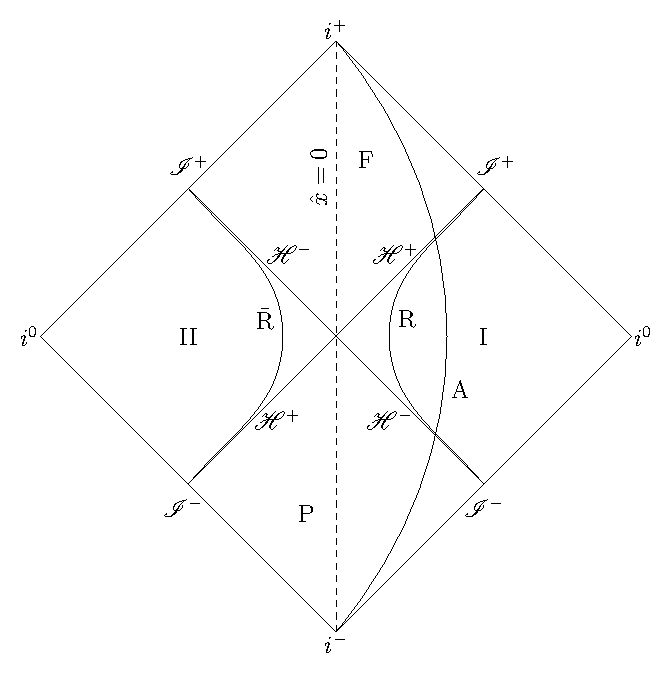
\includegraphics[width=.85\textwidth]{fig-rindler}
\caption{Flat spacetime conformal diagram showing Alice, Rob and AntiRob
trajectories. $i^0$ denotes the spatial infinities, $i^-$, $i^+$ are
respectively the timelike  past and future infinities,
$\mathscr{I}^-$ and $\mathscr{I}^+$ are the null past and future infinities
respectively, and $\mathscr{H}^\pm$ are the Rindler horizons.}
\end{center}
\label{Rindler}
\end{figure}
As usual, since the second partner (Rob) ---who  observes the bipartite state
\eqref{Min1}--- is accelerated, it is convenient to map the second partition
of this state  into the Rindler Fock space basis, which can be computed
using equations
\eqref{scavacinf1} and \eqref{unoinf1}.
\begin{equation}\label{Minscalar}
\ket\Psi_\text{s}=\sum_{n=0}^\infty \frac{(\tanh r_{\text{b}})^n}{\sqrt{2}
\cosh r_{\text{b}}} \bigg(\ket{0}_\text{A}
\ket{n_{\omegar}}_\text{I}\ket{n_{\omegar}}_{{\text{II}}}+\left.\frac{\sqrt{n+1}}{\cosh r_{\text{b}}}\ket{1}_\text{A}
 \ket{n+1_{\omegar}}_\text{I}\ket{n_{\omegar}}_{\text{II}}\right).
 \end{equation}
 
The same can be done in the case of a Dirac field. Let us now consider the
following maximally entangled state for a Dirac field in the Minkowskian
basis
\begin{equation}\label{Minf}
\ket{\Psi}_\text{d}=\frac{1}{\sqrt2}\left(\ket{0}\ket{0}+
\ket{\uparrow}_\text{A}\ket{\downarrow_\omegar}_\text{U}\right).
\end{equation}
As for the bosonic case, if Rob, who observes this bipartite state, is
accelerated, it is convenient to map the second partition of this state into
the Rindler Fock space basis, which can be computed using Eqns.
\eqref{vacuumf1} and \eqref{onepartf1}. The explicit form of such state
can be seen in chapter \ref{onehalf}.

Notice that we have chosen a specific maximally entangled state
\eqref{Minf} of all the possible choices. This election has no relevance
since in previous chapters it was shown the universality of the degradation of
fermionic entanglement. All fermionic maximally entangled states are
equally degraded by the Unruh effect, no matter what kind of maximally
entangled state is (either occupation number or spin Bell state), or even if
we work with a Grassmann scalar field instead of a Dirac field.

Let us denote
\begin{equation}\label{dens}
\rho^\text{s}_{\text{AR}\bar{\text{R}}}=\proj{\Psi_\text{s}}{\Psi_\text{s}},\qquad \rho^\text{d}_{\text{AR}\bar{\text{R}}}=\proj{\Psi_\text{d}}{\Psi_\text{d}},
\end{equation}
the tripartite density matrices for the bosonic and fermionic cases,  in
which we use the Minkowski basis for Alice and the Rindler basis for
Rob-AntiRob.

In the standard Unruh entanglement degradation scenario we must trace over AntiRob degrees of freedom when accounting
for the quantum state shared by Alice and Rob. This provokes, for
instance, the observation of a thermal bath by Rob while Alice observes
the Minkowski vacuum as it can be seen elsewhere
(\cite{Birrell,AlsingSchul} and sections \ref{tue} and \ref{sec42m}). As a consequence the state becomes
mixed, which can cause some degree of correlation loss in the system AR as
we increase the value of the acceleration $a$. In references
\cite{Alicefalls,AlsingSchul,Ditta,DiracDiscord} and in previous chapters it was
studied how this phenomenon affects the entanglement for different
fields.

The correlation
trade-off among the all possible bipartitions of the system, 
 Alice-Rob (AR),  Alice-AntiRob $(\text{A}\bar{\text{R}})$, and
  Rob-AntiRob $(\text{R} \bar{\text{R}})$ It has been also studied in chapter \ref{etanthrough}.
  
 Classical communication between the two partners is only
allowed for the bipartitions AR and $\text{A}\bar{\text{R}}$. We refer to these bipartitions as  `Classical communication allowed'. These bipartitions are the only ones in which quantum information
tasks are possible.

On the other hand, no quantum information tasks can be performed using
$\text{R}\bar{\text{R}}$ correlations since classical communication
between Rob and AntiRob is not allowed. Anyway, studying this
bipartition is still necessary to give a complete description of the
behaviour of the correlation created between the spacetime regions
separated by the horizon.

The partial quantum states
for each bipartition are obtained by tracing over the third subsystem as usual
\begin{equation}\label{traza1}
\rho^{\text{AR}} = \tr_{{\text{II}}}\rho^{\text{AR}\bar{\text{R}}},\qquad \rho^{\text{A}\bar{\text{R}}} = \tr_{\text{I}}\rho^{\text{AR}\bar{\text{R}}},\qquad \rho^{\text{R}\bar{\text{R}}}=\tr_{\text{A}}\rho^{\text{AR}\bar{\text{R}}}.
\end{equation}

The properties of the correlations among these
subsystems have been analysed in previous chapters, showing a completely
different behaviour of quantum correlations for the CCA bipartitions
depending on whether the system is fermionic or bosonic.

For fermionic fields we saw that quantum correlations are conserved as Rob
accelerates (see subsection \ref{conservanet}). Specifically, as entanglement in the
bipartition AR is reduced, entanglement in the system
$\text{A}\bar{\text{R}}$ is increased. In the limit of
$a\rightarrow\infty$ some entanglement survives in all the bipartitions of
the system.

For the scalar field the situation is radically different, namely, no
entanglement is created in the CCA bipartitions (see subsection \ref{negatsecm4}). Moreover, the
entanglement in the AR bipartition is very quickly lost as Rob accelerates,
even if we artificially limit the dimension of the Hilbert space
(see chapter \ref{boundedpop}).

We have seen that this different behaviour is only ruled by statistics, which
plays a crucial role in the phenomenon of Unruh entanglement
degradation. The role of statistics is so important that, for fermions, the
behaviour of quantum correlations has been proven to be universal. Also, the survival of entanglement for the fermionic case, is
arguably related to statistical correlations as we will see later. All these
aspects will be discussed in depth later on, when we present the results
for the Schwarzschild black hole.

\section{The ``Black Hole Limit'': from Rindler to Kruskal}\label{sec2m6}



In this section we will study a completely new setting using the tools
learned from previous chapters. We will prove in a
constructive way that the entanglement degradation in the vicinity of an
eternal black hole can be studied in detail with these well-known tools. By
means of the construction shown below we will be able to deal with new
problems such as computing entanglement loss between a free-falling
observer and another one placed at fixed distance to the event horizon as
a function of the distance, studying the behaviour of quantum
correlations in the presence of black holes.

To begin this section let us work a little bit with the Schwarzschild
metric
 \begin{equation}
 \diff s^2=-\left(1-\frac{2m}{r}\right)\diff t^2+\left(1-\frac{2m}{r}\right)^{-1}
 \diff r^2 +r^2\diff \Omega^2,
 \end{equation}
 where $m$ is the black hole mass and $\diff\Omega^2$ is the line element in the unit sphere.
Due to the symmetry of the problem we are going to restrict the analysis
to the radial coordinate. To shorten notation let us write the radial part
of metric as
 \begin{equation}\label{propsch}
 \diff s^2=-f\diff t^2+f^{-1}\diff r^2,
 \end{equation}
 where $f=1-2m/r$.

 We can choose to write the metric in terms of the proper time $t_0$ of an observer placed in $r=r_0$ as follows,
  \begin{equation}\label{propsch2}
 \diff s^2=-\frac{f}{f_0}\diff t_0^2+f^{-1}\diff r^2,
 \end{equation}
where $f_0=1-2m/r_0$.
The relationship between $t_0$ and $t$ is given by the norm of the
timelike Killing vector $\xi=\partial_t$ in $r=r_0$, namely
 $t_0=\sqrt{f_0}\,t$.

We can now change the spatial coordinate such that the new coordinate
vanishes at the Schwarzschild radius $r=R_{\text{b}}=2m$. Let us define
$z$ in the following way
 \begin{equation}\label{defz}
 r-2m=\frac{z^2}{8m}\quad\Rightarrow\quad
  f=\frac{(\kappa z)^2}{1+(\kappa z)^2},
 \end{equation}
 with $\kappa =1/(4m)$ being the surface gravity of the black hole. Then the metric \eqref{propsch2} results
 \begin{equation}\label{change1}
 \diff s^2=-\frac{1}{f_0}\frac{(\kappa z)^2}{1+(\kappa z)^2}\diff t_0^2+
 \left[1+(\kappa z)^2\right]\diff z^2.
 \end{equation}
Near the event horizon ($z\approx0$), we can expand this metric to
lowest order in $z$ and approximate it by
%\begin{equation}{1+(\kappa z)^2}\approx 1\end{equation}
%Therefore, the metric can be approximated in this region by
\begin{equation}\label{misli}
\diff s^2=-\left(\frac{\kappa z}{\sqrt{f_0}}\right)^2\diff t_0^2+\diff z^2,
\end{equation}
which is a Rindler metric with acceleration parameter
$\kappa/\sqrt{f_0}$.

  On the other hand, Eq. \eqref{misli} represents
the metric near the event horizon in terms of the proper time of an
observer placed at $r=r_0$. The next step is giving a physical meaning to
this Rindler-like acceleration parameter. For this, we need to compute the
proper acceleration of a Schwarzschild observer placed at $r=r_0$,
which is, indeed, different from $\kappa$ (as $\kappa$ would be the
acceleration of an observer arbitrarily close to the horizon as seen from
a free-falling frame).

To compute $a$ for this observer as seen by himself (proper
acceleration) we must start from the Schwarzschild metric. The value of
the proper acceleration for an accelerated observer at arbitrary fixed
position $r$ is $a=\sqrt{a_\mu a^\mu}$ where $a^\mu=v^\nu\nabla_\nu
v^\mu$ is the observer 4-acceleration at such position, whereas $v^\mu$
is his 4-velocity.

The 4-velocity for a Schwarzschild observer in an arbitrary position $r$
is
\begin{equation}
v^\mu= {\xi^\mu}/{|\xi|},
\end{equation}
where $\xi\equiv\partial_t$ is the Schwarzschild timelike Killing vector.
As $\xi^\mu=(1,0,0,0)$ in Schwarzschild coordinates, 
$|\xi|=\sqrt{|g_{00}|}=\sqrt{f}$, and therefore
$v^\mu=\xi^\mu/\sqrt{f}$. Thus, we can compute the acceleration
4-vector
\begin{equation}
a^\mu=v^\nu\nabla_\nu v^\mu=\frac{1}{|\xi|}\xi^\nu\nabla_\nu
 \frac{\xi^\mu}{|\xi|} .
\end{equation}
Taking into account that $\xi^\mu$ is a Killing vector and, therefore, it
satisfies $\nabla_\mu\xi_\nu+\nabla_\nu\xi_\mu=0$, we easily obtain
\begin{equation}
a_\mu=\frac12\frac{\partial_\mu|\xi|^2}{|\xi|^2} =
 \frac{\partial_\mu f}{2f}=\frac{1}{2f}\left(0,\partial_r f ,0,0\right).
\end{equation}
Hence, since $g^{rr}=f$, the   proper acceleration for this observer is
\begin{equation}\label{properpropera}
a=\sqrt{g^{\mu\nu}a_\mu a_\nu}=\sqrt{\frac{(\partial_r f)^2}{4f} } .
\end{equation}
For an observer placed at $r=r_0$,
\begin{equation}\label{properpropera3}
a_0=\frac{\kappa}{\sqrt{f_0}}(1-f_0)^2.
\end{equation}

We know from \eqref{defz} that $1-f_0=[1+(\kappa z_0)^2]^{-1}$. So,
if the observer in $r=r_0$ is close to the event horizon ($r_0\approx
R_{\text{b}}$), then, to lowest order, $1+(\kappa z_0)^2\approx 1$ and
\begin{equation}\label{properproperaf}
a\approx {\kappa}/{\sqrt{f_0}}.
\end{equation}
Therefore, under this approximation, we can re-write \eqref{misli} as
\begin{equation}\label{Rindleradapt}
\diff s^2=-\left(a_0 z\right)^2\diff t_0^2+\diff z^2.
\end{equation}
This shows that the Schwarzschild metric can be approximated, in the
proximities of the event horizon, by a Rindler metric whose acceleration
parameter is the proper acceleration of an observer resisting in a position
$r_0$ close enough to the event horizon.

This approximation holds if
\begin{equation}\label{conditioaproximatio}
\left(\frac{z_0}{2R_{\text{b}}}\right)^2\ll1
\end{equation}
or, in other words, if
\begin{equation}\label{conditioaproximatio2}
\frac{\Delta_0}{R_\text{S}}\ll1,
\end{equation}
where $\Delta_0\equiv r_0-R_\text{S}$ is the coordinate distance from $r_0$ to
the event horizon. In the limit $r_0\rightarrow R_{\text{b}}$ we obtain
that $f_0\rightarrow0$ and, from \eqref{properproperaf},
$a_0\rightarrow\infty$. This shows rigorously that being very close to
the event horizon of a Schwarzschild black hole can be very well
approximated by the infinite acceleration Rindler case, as it was
suggested in \cite{Alicefalls,AlsingSchul}. This also enables us
to study what would happen  with the entanglement between observers
placed at different distances of the event horizon as far as the Rindler
approximation holds.

Now let us identify again who is who in this new scenario. For this, we
introduce the null Kruskal-Szeckeres coordinates
\begin{equation}\label{eq:szeckeres}
u=-\kappa^{-1}\exp[-\kappa (t-r^*)],\quad v=\kappa^{-1}\exp[\kappa (t+r^*)],
\end{equation}
where $r^*=r+2m\log|1-r/2m|$. In terms of these coordinates the radial
part of the Schwarzschild metric is
\begin{equation}
\diff s^2=\frac{-1}{2\kappa r}e^{-2\kappa r}\diff u\diff v,
\end{equation}
where $r$ is implicitly defined by (\ref{eq:szeckeres}). The Penrose
diagram for the maximal analytic extension of Schwarzschild spacetime obtained from these coordinates is shown in fig.~\ref{Kruskal}. In this coordinates, 
near the horizon the metric can be written to  lowest order as
\begin{equation}
\diff s^2=-e^{-1}\diff u \diff v
\end{equation}
and $uv=-(\kappa z)^2$.

\begin{figure}[h]
\begin{center}
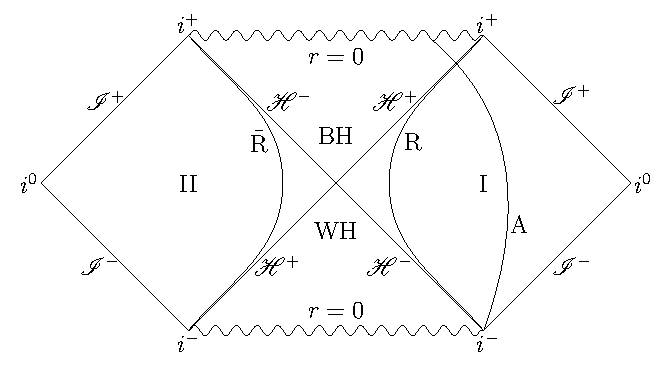
\includegraphics[width=.85\textwidth]{fig-kruskal}
\caption{Kruskal spacetime  conformal diagram showing trajectories for Alice,
Rob and AntiRob. $i^0$ denotes the spatial infinities, $i^-$, $i^+$
are respectively the timelike past and future infinities,
$\mathscr{I}^-$ and $\mathscr{I}^+$ are the null past and future infinities
respectively, and $\mathscr{H}^\pm$ are the event horizons.}
\label{Kruskal}
\end{center}
\end{figure}

Hence, there are three regions in which we can clearly define physical
timelike vectors respect to which we can classify positive and negative
frequencies:
\begin{itemize}
\item  $\partial_{\hat t}\propto (\partial_{u}+\partial_{v})$.
The parameter $\hat t$ for this timelike vector corresponds to the
proper time of a free-falling observer close to the horizon, and it is
analogous to the Minkowskian   timelike Killing vector. Positive
frequency modes associated to this timelike vector define a vacuum
state known as the Hartle-Hawking vacuum $\ket{0}_\text{H}$,
which is analogous to $\ket{0}_\text{M}$ in the Rindler case.


\item $\partial_{t}\propto (u\partial_{u}-v\partial_{v})$.
 This is the Schwarzschild timelike Killing vector, which (when properly
normalised) corresponds to an observer whose acceleration at the
horizon equals the surface gravity $\kappa$ of the black hole with
respect to a Minkowskian observer, or, in other words, with proper
acceleration $a_0\approx\kappa/\sqrt{f_0}$ close to the horizon.
The vacuum state corresponding to positive frequencies associated to
this timelike Killing vector is called the Boulware vacuum
$\ket{0}_\text{B}$. This state is analogous to the Rindler vacuum
$\ket{0}_\text{I}$.

\item There is another timelike Killing vector $-\partial_{t}$
(as in Rindler) for region II that will allow us to define another
Boulware vacuum  in region II. We will call it AntiBoulware vacuum
$\ket0_{\bar{\text{B}}}$, analogous to $\ket{0}_\text{II}$ in the
Rindler case.
\end{itemize}

Now, in this scenario,
$\ket{1_{\hat\omega}}_\text{H}=a^\dagger_{\hat\omega,\text{H}}\ket{0}_\text{H}$
are free scalar field modes, in other words, solutions of positive
frequency ${\hat\omega}$ with respect to $\partial_{\hat t}$  of the
free Klein-Gordon equation close to the horizon
\begin{equation}
\ket{1_{\hat\omega}}_\text{H}\equiv u_{\hat\omega}^\text{H}\propto
\frac{1}{\sqrt{2\hat\omega}}e^{-i\hat\omega \hat t}.
\end{equation}
The label H just means that those states are expressed in the
Hartle-Hawking Fock space basis.

An observer located at a fixed distance from the black hole can also define his own vacuum and
excited states of frequency $\omega$ respect to the Killing vector
$\partial_{t}$. Actually, there are two natural vacuum states associated
with the positive frequency modes in both sides of the horizon these are
$\ket{0}_\text{B}$ and $\ket{0}_{\bar{\text{B}}}$, vacua for the
positive frequency modes in regions I and II respectively (fig.
\ref{Kruskal}). Subsequently, for a scalar field, we can define the field
excitations as
\begin{align}
\ket{1_\omega}_{\text{B}}&=a^\dagger_{\omega,\text{B}}\ket{0}_\text{B}\equiv
u_\omega^{\text{B}}\propto\frac{1}{\sqrt{2\omega}}e^{-i\omega  t},\nonumber\\
\ket{1_\omega}_{\bar{\text{B}}}&=a^\dagger_{\omega,\bar{\text{B}}}
\ket{0}_{\bar{\text{B}}}\equiv u_\omega^{\bar{\text{B}}}\propto\frac{1}{\sqrt{2\omega}}e^{i\omega  t}.
\end{align}


%reeescribir
Then, the analogy between the Rindler-Minkowski and the Boulware-Hartle-Hawking states,  and their relation with 
the standard Alice-Rob-AntiRob notation is as follows:
\begin{equation}\label{identif}
\begin{array}{lclcl}
\ket{0}_\text{R}&\leftrightarrow&\ket{0}_\text{I}&\leftrightarrow&\ket{0}_\text{B},\\
\ket{0}_{\bar{\text{R}}}&\leftrightarrow&\ket{0}_{\text{II}}&
\leftrightarrow&\ket{0}_{\bar{\text{B}}},\\
\ket{0}_{\text{A}}&\leftrightarrow&\ket{0}_\text{M}&\leftrightarrow&
\ket{0}_{\text{H}}.
\end{array}
\end{equation}
The change of basis between Hartle-Hawking modes
and Boulware modes is completely analogous to the change of basis
between Minkowskian modes and Rindler modes with an acceleration
parameter $a_0=\kappa/\sqrt{f_0}$.

In the same fashion as for Rindler we define an orthonormal basis 
%\begin{equation}\label{HHs}
%\psi^\text{H}_{\omega_j}=\sum_i C_{ij}\, u^{\text{H}}_{\hat\omega_i}\qquad \psi'^{\text{H}}_{\omega_j}=\sum_i C'_{ij}\, u^{\text{H}}_{\hat\omega_i}\
%\end{equation}
of Hartle-Hawking scalar field modes $\{\psi^\text{H}_{\omega_j},\psi'^{\text{H}}_{\omega_j}\}$ whose elements are superpositions of  positive-frequency solutions
$u_{\hat\omega_i}^\text{H}$ of the Klein-Gordon equation with
respect to the Kruskal time $\hat t$
 such that each element  corresponds to Boulware modes of one single frequency in the Kruskal regions I and II
($u^\text{B}_{\omega_j}$ and $u^{\bar{\text{B}}*}_{\omega_j}$). The same can be
done for the Dirac field.
%\begin{equation}\label{HHf}
%\psi^\text{H}_{\omega_j,\sigma}=\sum_i D_{ij}\, u^{\text{H}}_{\hat\omega_i,\sigma}
%\qquad \bar \psi^\text{H}_{ \omega_j,\sigma}=\sum_i E_{ij}\,
%v^{\text{H}}_{\hat\omega_i,\sigma}.
%\end{equation}

We can express the Hartle-Hawking vacuum state in terms of the
Boulware Fock space basis.  To do so, we use what we learned from the
Rindler case. Taking into account that $\ket{0}_\text{H}=\bigotimes_{
i}\ket{0_{\omega_i}}_\text{H}$, we have that
\begin{equation}\label{scavacinf}
\ket{0_{\omega_i}}_\text{H}=\frac{1}{\cosh q_{\text{b},\omega_i}}
\sum_{n=0}^\infty (\tanh q_{\text{b},\omega_i})^n  \ket{n_{\omega_i}}_\text{B}
\ket{n_{\omega_i}}_{{\bar{\text{B}}}},
\end{equation}
where
\begin{equation}\label{defr3}
\tanh q_{\text{b},\omega_i}=\exp\left({-\pi \sqrt{f_0}\,\omega_i/{\kappa}}\right)
%=\exp\left[{-4\pi \omegar \sqrt{m^2-\dfrac{2m^3}{r_0}}}\right]
.
\end{equation}
The unprimed Hartle-Hawking one particle state in the basis $\{\psi^\text{H}_{\omega_j},\psi'^{\text{H}}_{\omega_j}\}$ results
from applying the corresponding creation operator to the vacuum state.
We can also translate this state to the Boulware basis:
  \begin{equation}\label{unoinf}
\ket{1_{\omega_i}}_\text{H} = \frac{1}{(\cosh q_{\text{b},\omega_i})^2}\sum_{n=0}^{\infty} (\tanh  q_{\text{b},\omega_i})^n\sqrt{n+1}
\ket{n+1_{\omega_i}}_\text{B}\!\ket{n_{ \omega_i}}_{{\bar{\text{B}}}}.
\end{equation} 

The Hartle-Hawking  vacuum (projected onto the unprimed sector) for the Dirac case is expressed in the
Boulware basis as follows
\begin{align}\label{vacuumf}
 \ket{0_{\omega_i}}_{\text{H}} &= (\cos q_{\text{f},\omega_i})^2
 \bikete{0_{\omega_i}}{0_{\omega_i}}
 +\sin q_{\text{f},\omega_i}\cos q_{\text{f},\omega_i}
 \left(\ket{\uparrow_{\omega_i}}_{{\text{B}}}
  \ket{\downarrow_{\omega_i}}_{\bar{\text{B}}}+
 \bikete{\downarrow_{\omega_i}}{\uparrow_{\omega_i}}\right)
 \nonumber\\
 &+(\sin q_{\text{f},\omega_i})^2\bikete{\pa_{\omega_i}}{\pa_{\omega_i}},
\end{align}
whereas the projected Hartle-Hawking one particle state 
is expressed in the Boulware basis as
\begin{align}\label{onepartf}
 \ket{\uparrow_{\omega_i}}_\text{H}&= \cos q_{\text{f},\omega_i}
 \bikete{\uparrow_{\omega_i}}{0_{\omega_i}}+
 \sin q_{\text{f},\omega_i}\bikete{\pa_{\omega_i}}{\uparrow_{\omega_i}},\nonumber\\
\ket{\downarrow_{\omega_i}}_\text{H}&=
\cos q_{\text{f},\omega_i} \bikete{\downarrow_{\omega_i}}{0_{\omega_i}}-
\sin q_{\text{f},\omega_i}\bikete{\pa_{\omega_i}}{\downarrow_{\omega_i}},
\end{align}
where this time
\begin{equation}\label{defr4}
\tan q_{\text{f},\omega_i}=\exp\left(-\pi \sqrt{f_0}\,\omega_i /{\kappa}\right)
%=\exp\left[{-4\pi \omegar \sqrt{m^2-\dfrac{2m^3}{r_0}}}\right]
.
\end{equation}

Thus, in this new scenario, we can consider a bipartite states for fermions and bosons analogous to
the states \eqref{Min1} and \eqref{Minf} for the Rindler scenario, which have the following form in the basis of a free-falling observer (Alice)
\begin{align}\label{Haw1}
\ket\Psi_\text{s}&=\frac{1}{\sqrt{2}}
\left(\ket{0}\ket{0}+
\ket{1}_\text{A}\ket{1_{\omegar}}_\text{H}\right),\\*
\label{Hawf}
\ket{\Psi}_\text{d}&=\frac{1}{\sqrt2}\left(\ket{0}
\ket{0}+\ket{\uparrow}_\text{A}
\ket{\downarrow_{\omegar}}_\text{H}\right).
\end{align}
This bipartite system consists in two subsystems, the first one is going to
be observed by Alice, who is free-falling into the black hole and close to
the event horizon, and the second one will be observed by Rob, who is near
the event horizon at $r=r_0\approx R_\text{S}$. Therefore, the second
partner who observes the bipartite states
\eqref{Haw1} and \eqref{Hawf}  describes \eqref{Haw1} and  \eqref{Hawf} using the Boulware
basis, so that it is convenient to map the second partition of these states
into the Boulware Fock space basis.

Following the notation \eqref{identif}, to analyse the correlations among
the bipartite subsystems we need to trace out the third subsystem
analogously to what we did in \eqref{traza1}:
\begin{eqnarray}\label{traza2}
\nonumber\rho^{\text{AR}}&\!\!=\!&\tr_{{\text{II}}}\rho^{\text{AR}\bar{\text{R}}},\\*
\nonumber\rho^{\text{A}\bar{\text{R}}}&\!\!=\!&\tr_{\text{R}}\rho^{\text{AR}\bar{\text{R}}},\\*
\rho^{\text{R}\bar{\text{R}}}&\!\!=\!&\tr_{\text{A}}\rho^{\text{AR}\bar{\text{R}}}.
\end{eqnarray}

It can be seen in fig. \ref{Kruskal} that all the information beyond the
event horizon cannot be accessed by Rob. Actually, what happens beyond
the horizon is determined by the information that Rob can access along
with the information that AntiRob can access. In this context it makes
sense to say that studying the system $\rho^{\text{R}\bar{\text{R}}}$
gives an idea of the correlations across the horizon.



\section{Correlations behaviour}\label{sec4}

In this section we will use the machinery we already have from the Rindler
set-ups to compute the entanglement degradation as a function of the
position of Rob.

First we will consider that Rob's frequency $\omegar$ is measured in
natural units adapted to each black hole. This will show how modes of
different frequencies  suffer different correlation degradation. It will
also show how less massive black holes produce a higher degradation than
the heavier ones. Furthermore, this analysis will show the universality of
the phenomenon of the Hawking entanglement degradation for
Schwarzschild black holes.

After that, we will  analyse the different degree of entanglement
degradation experimented by an observer of fixed Boulware frequency
$\omegar$ standing at fixed distances from the event horizon for
different black hole masses.

In the following subsections we will see that all the interesting behaviour
happens in regions in which the Rindler approximation
\eqref{Rindleradapt} is valid. Specifically, we will see in the plots below that the
values of the distance to the horizon where the interesting
entanglement behaviour appears are in the regime $\Delta_0\lesssim 0.05R_\text{S}$
in all the cases considered in this section for which, consequently, the
approximation \eqref{Rindleradapt} holds.

\subsection{Adapted frequency}

In terms of the mode frequency measured by Rob  (written in units
natural to the black hole, i.e. in terms of the surface gravity $\kappa$) and his position measured in Schwarzschild
radii,
\begin{align}
\Omega&=2\pi\omegar
/\kappa=8\pi m\omegar,\\
R_0&=r_0/R_\text{S}=r_0/(2m),
\end{align}
 Eqns. \eqref{defr3} and
\eqref{defr4} can be written as
\begin{align}\label{defr32}
\tanh q_\text{s}&=\exp\left({-\frac{\Omega}{2} \sqrt{1-\frac{1}{R_0}}}\right),
\\
\label{defr42}
\tan q_\text{d}&=\exp\left({-\frac{\Omega}{2} \sqrt{1-\frac{1}{R_0}}}\right),
\end{align}
showing that the phenomenon of Hawking entanglement degradation
presents universality, which is to say, if the frequency is measured in natural
units, every Schwarzschild black hole behaves in the same way, as
expected.

\subsubsection{Quantum correlations}

We will use the negativity ($\mathcal{N}$) to account for the quantum
correlations between the different bipartitions of the system. Hence, to compute it, we will need the partial transpose of the bipartite
density matrices \eqref{traza2}. The details associated to the
diagonalisation of the partial transposed density matrices for each
subsystem are technically very similar to the Rindler case, and are not of
much interest for the purposes of this article. All the technical aspects of
such calculations can be found in chapter \ref{etanthrough} for Dirac and scalar fields.
The results of those calculations are shown in Figs. \ref{sncca} to
\ref{dnrar}. In Figs. \ref{sncca} and \ref{dncca} we can see the behaviour
of the negativity on the CCA bipartitions for different values of Rob's
frequency $\Omega$.



For the scalar field we can see that as Rob is closer to the event horizon
the entanglement shared between Alice and Rob decreases. In the limit in
which Rob is very close to the horizon, entanglement is completely lost.
With the study performed here we can see the functional
dependence of the entanglement with the distance to the horizon. As seen in the figures,
 the degradation phenomenon occurs in a narrow region very close
to the event horizon. If Rob is far enough from the black hole he will not
appreciate any entanglement degradation effects unless either the mass of the black hole or the frequency of the mode considered are extremely small. There must be, indeed, a minimum residual effect associated to the Hawking thermal bath experienced in the asymptotically flat region of the spacetime, far from the region in which this approximation is valid, but it is unnoticeably small. Certainly, as it will be seen in fig. \ref{realb} and the discussion below, even very close to the horizon no effective entanglement degradation 
 occurs for physically meaningful values of mass and frequency.  
 
If we keep the frequency measured by Rob $(\omegar)$ constant,
$\Omega$ will grow proportional to  the black hole mass. With this in
mind, fig. \ref{sncca} shows that the degradation is stronger for less
massive black holes. This result is consistent with the fact that the
Hawking temperature increases as the mass of the black hole goes to
zero. In the next section (specifically in fig. \ref{realb}) we will show
that this is not an effect of choosing natural units, when an observer is at
a fixed distance of a black hole, the degradation will be higher for less
massive black holes.

\begin{figure}[h]
\begin{center}
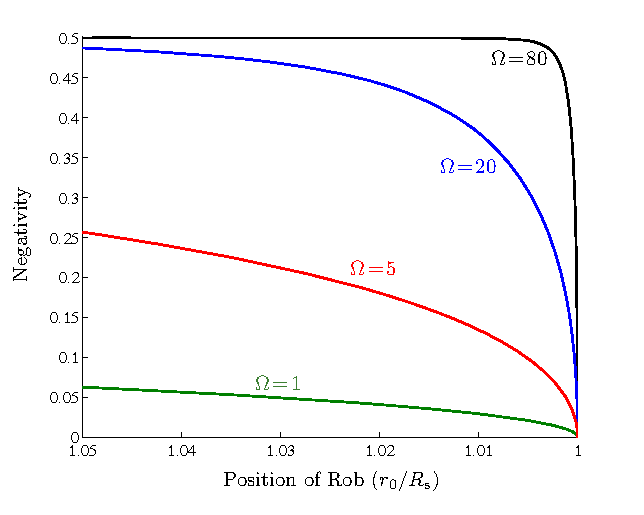
\includegraphics[width=.85\textwidth]{arboswa}
\caption{Scalar field: Entanglement of the system Alice-Rob as a function of the position of Rob for different values of $\Omega$. Entanglement vanishes as Rob approaches
the Schwarzschild radius while no entanglement is created between Alice and AntiRob. The smaller the value of $\Omega$ the more degradation is produced by the black hole.}
\label{sncca}
\end{center}
\end{figure}

In any case, for the scalar field, the entanglement in the system AR is
completely degraded when one of the observers is resisting very close to
the event horizon of the black hole. Hence, in this scenario, no quantum
information resources can be used (for instance to perform quantum
teleportation or quantum computing) between a free-falling observer and
an observer arbitrarily close to an event horizon. Moreover, no
entanglement of any kind is created among the CCA bipartitions of the
system (the ones where classical communication is allowed). Therefore, all useful
quantum correlations between a free-falling observer and an observer at
the event horizon are lost due to the Hawking effect degrading all the
entanglement in the system.



For the Dirac field  (fig. \ref{dncca}) something very different happens.
We see that correlations in the bipartition AR decrease to a certain
finite limit, which means that there is entanglement survival even when
Rob is asymptotically close to the event horizon. This survival is a well
known phenomenon in the Rindler case \cite{AlsingSchul}. At the
same time that entanglement is destroyed in the AR bipartition,
entanglement is created in the complementary $\text{A}\bar{\text{R}}$
bipartition so that negativity in the CCA bipartitions fulfils a
conservation law regardless of the distance to the event horizon and the
mass of the black hole
\begin{equation}\label{conservan}
\mathcal{N}_\text{AR}+\mathcal{N}_{\text{A}\bar{\text{R}}}=\frac12.
\end{equation}
The nature of this entanglement and the survival of correlations, even in
the limit of positions arbitrarily close to the horizon, is discussed in chapters \ref{etanthrough} and \ref{boundedpop} for the Rindler case. When we deal with fermionic
fields there are correlations that come from the statistical fermionic
nature of the field which we cannot get rid of. The hypothesis is that this
entanglement, which is purely statistical, is the second quantised version
of the statistical entanglement disclosed in \cite{sta1}. Here we see that
the same conclusions drawn in that case can be perfectly applied to the
Schwarzschild black hole case.

\begin{figure}[h]
\begin{center}
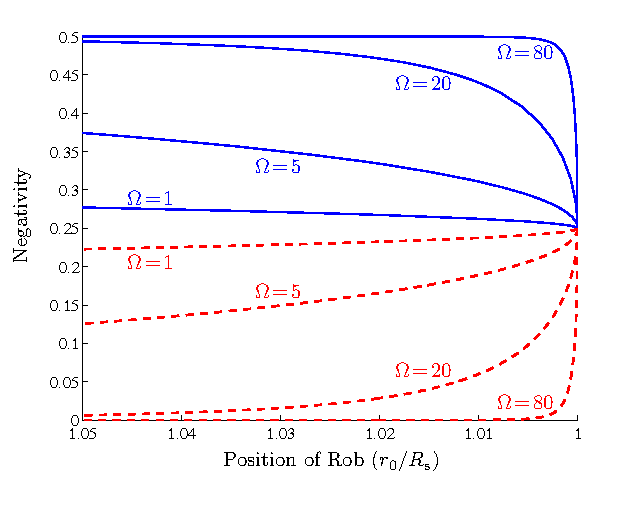
\includegraphics[width=.85\textwidth]{negativityCCA}
\caption{Dirac field: Entanglement Alice-Rob (blue solid line) and
Alice-AntiRob (red dashed line). Universal conservation law for fermions
is shown for different values of $\Omega$. The entanglement
degradation in AR is quicker when $\Omega$ is smaller. The maximum
degradation is not total and its value is independent of $\Omega$.
}
\label{dncca}
\end{center}
\end{figure}

About the dependence of the entanglement degradation on the frequency
of the Boulware mode, Fig. \ref{sncca}  shows that, for a scalar field, the
loss of entanglement between a free falling observer and an observer
outside but very close to the event horizon (AR) is greater for modes of
lower frequency. This makes sense because, energetically speaking, it is
cheaper to excite those modes and, therefore, they are more sensitive to
the Hawking thermal noise. For a Dirac field (Fig. \ref{dncca}) we see a
similar behaviour. However, the surviving
entanglement in the limit in which Rob is infinitely close to the event
horizon is not sensitive to the frequency of the mode considered;
remarkably,  the entanglement decays down to the same finite value for all
modes. This is in line with the idea that the entanglement that survives the
event horizon is merely due to statistical correlations,  and the only
information that survives when Rob is exactly at the horizon is the fact
that the field is fermionic as suggested in chapter \ref{etanthrough}.




From Figs. \ref{sncca} and \ref{dncca} we can also conclude that all the
relevant entanglement degradation phenomena is produced in the
proximities of the event horizon so that the Rindler approximation that
we are carrying out is valid  (Eq. \ref{conditioaproximatio2}). We can also
see that the degradation is small even in regions in which the
approximation  still holds. Therefore for longer distances from the
horizon the presence of event horizons is not expected to perturb
entangled systems.

\begin{figure}[h]
\begin{center}
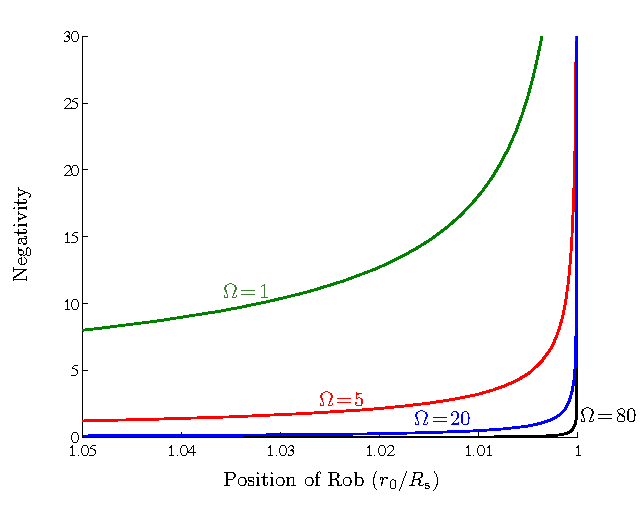
\includegraphics[width=.85\textwidth]{rarboslm}
\caption{Scalar field: Entanglement of the system Rob-AntiRob
(entanglement between regions I and II) as a function of the position of
Rob for different values of $\Omega$. Entanglement diverges as Rob
approaches   the Schwarzschild radius.}
\label{snrar}
\end{center}
\end{figure}

In Figs. \ref{snrar} and \ref{dnrar} we can see the behaviour of the
negativity on the $\text{R}\bar{\text{R}}$ bipartition for scalar and
Dirac fields respectively. Here we see that quantum correlations between I and II are created as Rob is standing closer to the event horizon. In
other words,  as Rob is getting closer to the event horizon the partial
system $\text{R}\bar{\text{R}}$ gains quantum correlations. This result
shows that, when Rob is near the horizon, the field states in both sides of
the event horizon are not completely independent. Instead, they get more
and more correlated. However, this $\text{R}\bar{\text{R}}$
entanglement is useless for quantum information tasks because classical
communication between both sides of an event horizon is forbidden. It is
well known for the Rindler case that quantum correlations are created
between Rob and AntiRob when the acceleration increases.
Here we see the direct translation to the Kruskal scenario. The growth of
those correlations encodes information about the dimension of the Fock
space for each field mode as seen in chapter \ref{boundedpop}.



\begin{figure}[h]
\begin{center}
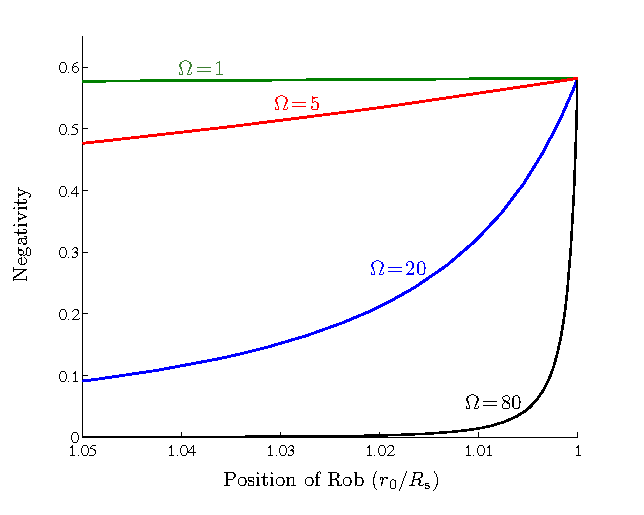
\includegraphics[width=.85\textwidth]{negaaarf}
\caption{Dirac field: Entanglement of the system Rob-AntiRob
(entanglement between regions I and II) as a function of the position of Rob for
different values of $\Omega$. Entanglement tends to a finite value as Rob
approaches   the Schwarzschild radius.}
\label{dnrar}
\end{center}
\end{figure}



%\begin{figure}[h]
%\begin{center}
%\includegraphics[width=.70\textwidth]{arbosw}
%\caption{(Scalar field: Entanglement of the system Alice-Rob as a function of the position of Rob for different $\omega$. Entanglement vanishes as Rob %approaches to the Schwarzschild radius. Black hole mass is fixed $m=1$}
%\label{Kruskal}
%\end{center}
%\end{figure}




\subsubsection{Mutual information}

To compute the
mutual information  for each bipartition we will need the eigenvalues of
the corresponding density matrices. Again the technicalities of this
analysis can be found in previous chapters. The results for the
CCA bipartitions are shown in Figs. \ref{smi} and \ref{dmi}.

\begin{figure}[h]
\begin{center}
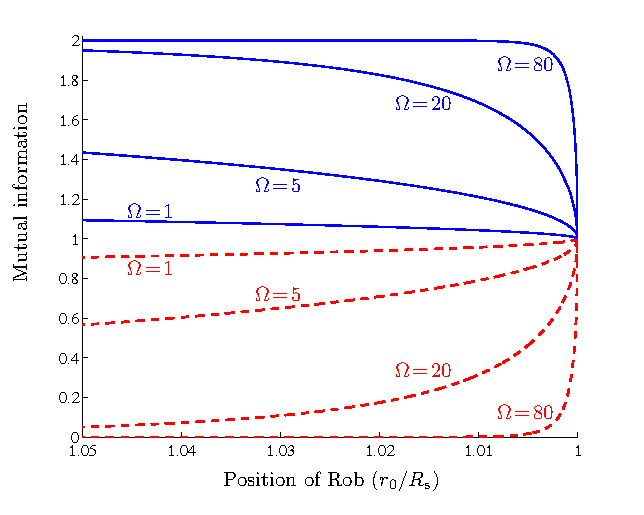
\includegraphics[width=.85\textwidth]{conservabos}
\caption{Scalar field: Mutual information Alice-Rob (blue solid line) and
Alice-AntiRob (red dashed line).  Mutual information  AR
decreases as Rob is closer to the horizon and mutual information
$\text{A}\bar{\text{R}}$ grows.}
\label{smi}
\end{center}
\end{figure}

\begin{figure}[h]
\begin{center}
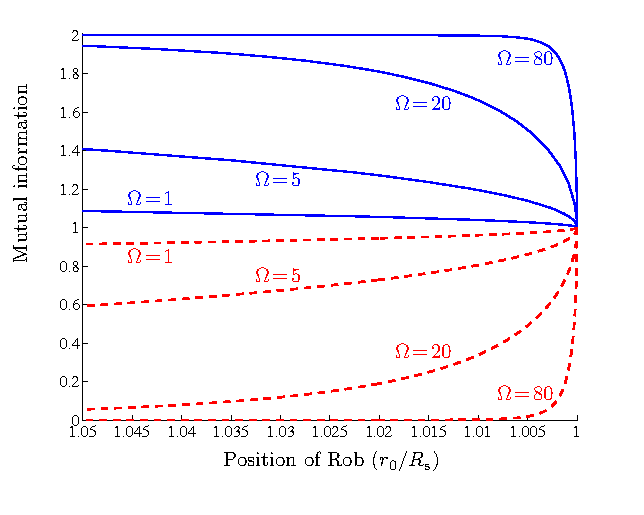
\includegraphics[width=.85\textwidth]{muinfer}
\caption{Dirac field: Mutual information Alice-Rob (blue solid line) and
Alice-AntiRob (red dashed line).  Mutual information  AR
 decreases as Rob is closer to the horizon and mutual information $\text{A}\bar{\text{R}}$
  grows.}
\label{dmi}
\end{center}
\end{figure}

We see here that we obtain the black hole version of the mutual
information universal conservation law found in previous chapters for the
Rindler case. Namely, for any distance to the horizon or
black hole mass it is fulfilled that
\begin{equation}\label{conservami}
I_\text{AR}+I_{\text{A}\bar{\text{R}}}=2.
\end{equation}
Although, as we can see by comparing Figs. \ref{smi} and  \ref{dmi}, the
behaviour of the mutual information is very similar for both fermions and
bosons, the origin of this conservation law near the event horizon is
completely different.

For scalar fields this conservation near the horizon responds to a
conservation of  classical correlations only. This can be deduced from Fig.
\ref{sncca} which shows that quantum correlations drop very quickly as
the distance of Rob to the horizon decreases and, consequently, the only
correlations left  must be classical. However, the conservation of
classical correlations in the CCA bipartitions has to do with the
infiniteness of the dimension of the Hilbert space, as it is shown in
chapter \ref{boundedpop}. If the dimension of a bosonic field is limited to a finite value,
classical correlations also drop  as Rob is closer to the horizon (as
quantum correlations do).

On the other hand, a Dirac field has a built-in dimensional limit for the
Hilbert space of each mode imposed by Pauli exclusion principle. Although
previous chapters demonstrated that this limit in the dimension has nothing
to do with the behaviour of quantum correlations, it
does limit the creation of classical correlations. Analogously to what is
discussed in chapter \ref{boundedpop}, the origin for the conservation law
(\ref{conservami}) in the fermionic case is a direct consequence of the
quantum correlations conservation law \eqref{conservan} while for scalar fields it responds to a conservation of
classical correlations.

Mutual information for the $\text{R}\bar{\text{R}}$ bipartition does
not add any new result as it inherits the quantum correlations behaviour
showed in figs. \ref{sncca} and \ref{dncca}.

\subsection{Entanglement degradation dependence on the black hole mass}

In this section we will analyse the entanglement degradation for an
observer with the same characteristics in the presence of  different
black holes. To do so we are going to use the full dimensional quantities
$\omegar$ and $\Delta_0$.

We will consider that Rob's mode frequency is $\omegar=1.5$ Mhz, and
he is standing at a distance $\Delta_0=1$ cm and $\Delta_0=10$ cm
from the event horizon of  black holes with different masses, while he
shares an entangled state
\eqref{Haw1} or \eqref{Hawf} with a free-falling observer Alice.

The quantum correlations that Rob and Alice share are shown in Figs.
\ref{realb} and \ref{realf} for scalar and Dirac fields, respectively.
From these figures we see that for a really close distance from the event
horizon, only small black holes would produce significant entanglement
degradation. Actually, the degradation decreases very quickly as the
black hole mass is increased.




\begin{figure}[h]
\begin{center}
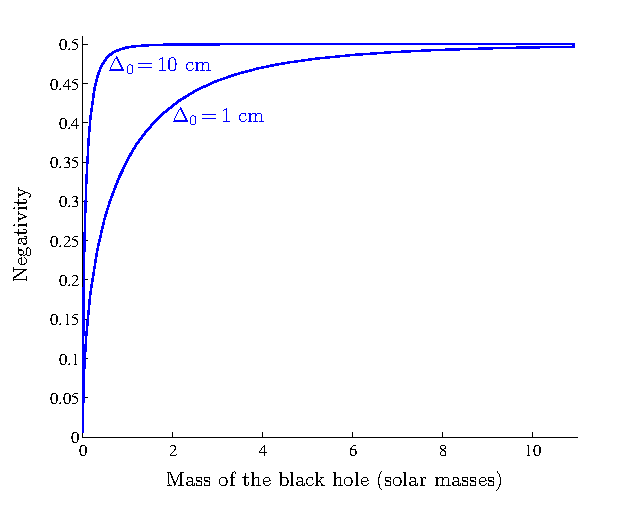
\includegraphics[width=.85\textwidth]{1cm1Mhz}
\caption{Scalar field: Entanglement Alice-Rob when Rob stands at a distance
of 1 cm and 10 cm from the event horizon for a fixed frequency
$\omegar=1.5$ Mhz as a function of the black hole mass. Notice that,
for these values of $\Delta_0$, the approximation holds perfectly for any mass $m>10^{-5}$ solar masses.}
\label{realb}
\end{center}
\end{figure}


\begin{figure}[h]
\begin{center}
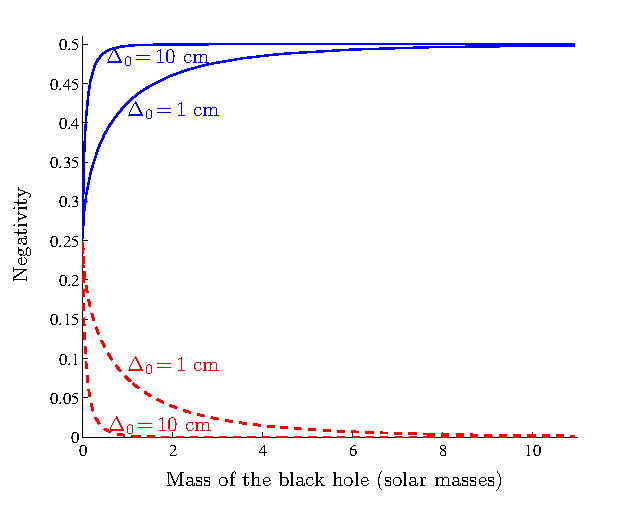
\includegraphics[width=.85\textwidth]{1cm1Mhzf}
\caption{Dirac field: Entanglement AR (blue continuous line) and
 $\text{A}\bar{\text{R}}$ (red dashed line) when Rob stands at a
 distance of 1 cm and 10 cm from the event horizon for a fixed frequency
  $\omegar=1.5$ Mhz as a function of the black hole mass.
  Notice that, for these values of $\Delta_0$, the approximation holds perfectly for any mass $m>10^{-5}$ solar masses.}
\label{realf}
\end{center}
\end{figure}


Furthermore, we can see that the effects on the entanglement decrease
very quickly as the distance to the event horizon is increased. This shows
that quantum information tasks can be safely performed in universes that
present event horizons since only in the closest vicinity of the less massive
black holes the Hawking effect impedes the application of quantum
information protocols.



\section{Localisation of the states}\label{newsec5}

Along this work we have used a plane-wave-like basis to express the quantum state of the field for the inertial an accelerated observers. These plane wave modes are completely delocalised, and therefore, they are not the most natural election of modes if we want to think of the observers Alice and Rob as spatially localised to some degree. We will present the method to build such states, although this topic will be more deeply treated in chapter \ref{sma}.

A very similar analysis to the one carried out in sections \ref{sec2m6} and \ref{sec2m6} can be performed using a complete set of wave packet modes for both the Minkowski and Rindler solutions of the wave equation. These modes can be spatially localised and provide a clearer physical interpretation for Alice and Rob, which will eventually have to carry out measurements on the field. The way to build these wave packet modes can be found in chapter \ref{sma} and, among many others, in \cite{Birrell,Takagi,NavarroSalas}.

The elements of this basis are defined as a function of the plane wave modes \eqref{modmin} as
\begin{equation}
u^{\text{M}}_{\hat\omega,l}=\frac{1}{\sqrt{\epsilon}}\int_{\hat \omega}^{\hat \omega+\epsilon}d\nu\, e^{-i \nu l}u^{\text{M}}_{\nu},
\end{equation}
where $\hat\omega$ and $l$ label each wave packet.
 
 We can define creation an annihilation operators associated to these wavepackets $a_{\hat \omega,l,\text{M}}$, $a_{\hat\omega,l,\text{M}}^\dagger$  such that $a_{\hat\omega,l,\text{M}}$ annihilates the Minkowski vacuum and $a_{\hat\omega,l,\text{M}}^\dagger \ket{0}_\text{M}=\ket{1_{\hat\omega,l}}_\text{M}$ represents a wavepacket peaked for a frequency $\hat \omega$ and whose spatial localisation can be associated to the maximum of $u^{\text{M}}_{\omega,l}$ as a function of $\hat x$ and $\hat t$.
 
A similar analysis can be done for the Rindler basis
\begin{align}
\nonumber u^{\text{I}}_{\omega,l'}&=\frac{1}{\sqrt{\epsilon}}\int_{\omega}^{ \omega+\epsilon}d\nu\, e^{-i \nu l'}u^{\text{I}}_{\nu},\\
u^{\text{II}}_{\omega,l'}&=\frac{1}{\sqrt{\epsilon}}\int_{\omega}^{ \omega+\epsilon}d\nu\, e^{-i \nu l'}u^{\text{II}}_{\nu},
\end{align}
 $\omega$ and $l'$ label each wave packet.  We can define creation an annihilation operators associated to these wavepackets $a_{\omega,l',R}$, $a_{\omega,l',R}^\dagger$ (where $R=\text{I},\text{II}$) such that $a_{\omega,l',R}$ annihilates the region Rindler region $R$ vacuum and $a_{\omega,l',R}^\dagger \ket{0}_R=\ket{1_{\omega,l'}}_R$ represents a wavepacket peaked for a Rindler frequency $\omega$ and whose spatial localisation can be associated to the maximum of $u^R_{\omega,l'}$ as a function of $x$ and $t$.
 
 We can compute then the Bogoliubov transformation between the Minkowski wavepackets and the Rindler wavepackets \cite{NavarroSalas}
 \begin{equation}
a_{\hat\omega,l,\text{M}}=\alpha^{\text{I}*}_{\omega,l',\hat \omega,l}\,
a^{\phantom{\dagger}}_{\omega,l',\text{I}}-\beta^{\text{II}*}_{\omega,l',\hat \omega,l}\,
a^\dagger_{\omega,l',\text{II}}.
\end{equation}
Where the Bogoliubov coefficients are computed in the same fashion as for the plane wave case
\begin{equation}
\alpha^{\text{I}}_{\omega,l',\hat \omega,l}=\left(u^{\text{I}}_{\omega,l'},u^{\text{M}}_{\hat\omega,l}\right),
\quad\beta^{\text{II}}_{\omega,l',\hat \omega,l}=-\left(u^{\text{II}}_{\omega,l'},u^{\text{M}*}_{\hat\omega,l}\right).
\end{equation}

It is shown in \cite{NavarroSalas} that, apart from an irrelevant phase factor, the Bogoliubov coefficients are related with \eqref{bogo1} as follows
\begin{align}\label{bogonew}
\nonumber\alpha^{\text{I}}_{\omega,l',\hat \omega,l}&=\hat\alpha^{\text{I}}_{ij}\,\mathcal{G}_\alpha(\hat\omega,l,\omega,l'),\\
\beta^{\text{I}}_{\omega,l',\hat \omega,l}&=\hat\beta^{\text{II}}_{ij}\,\mathcal{G}_\beta(\hat\omega,l,\omega,l').
\end{align}
It is shown in \cite{NavarroSalas} that $\mathcal{G}_\alpha(\hat\omega,l,\omega,l')\approx \delta_{\omega\omega_\alpha}\delta_{ll_\alpha}$ and  $\mathcal{G}_\beta(\hat\omega,l,\omega,l')\approx \delta_{\omega\omega_\beta}\delta_{ll_\beta}$, where $l_\alpha=l_\alpha(l')$ and $\omega_\alpha =\omega_\alpha( \omega,l')$.

The key feature of this transformations is that they have again a diagonal form. As it can be read from \eqref{bogonew}, a Minkowski wavepacket $\ket{1_{\omega,l'}}_\text{M}$ is connected with a pair of Rindler wavepackets in regions I and II. Moreover, the functional form of the dependence of this coefficients with the acceleration is effectively the same. This analysis made for the Rindler and Minkowskian modes can be straightforwardly translated to the Boulware and Hartle-Hawking modes.  A completely analogous analysis can be done for the fermionic case.

Consequently all the conclusions extracted in this article for delocalised modes are also valid for the localised modes defined above.

\section{Discussion}\label{conclusions}


We have analysed the entanglement degradation produced in the vicinity
of a Schwarzschild black hole.

With this aim, we have carried out a detailed study of the Schwarzschild
metric in the proximity of the horizon, showing how we can adapt the
tools developed in the study of the entanglement degradation for
uniformly accelerated observers
to the black hole case. In particular, we have shown that, regarding
entanglement degradation effects, the Rindler limit of infinite acceleration reproduces
a black hole scenario in which Rob is arbitrarily close to the event horizon.
More importantly, we have shown the fine structure of this  limit, making
explicit the dependence of the entanglement degradation phenomena on the distance
to the horizon, the mass of the black hole, and the Boulware frequency
$\omegar$ of the entangled mode under consideration, while keeping
control of the approximation to make sure that the toolbox developed for
the Rindler case can be still rigorously used here.

By means of this analysis we have seen that all the interesting
 entanglement degradation phenomena due to the Hawking effect are produced very
close to the event horizon of the Schwarzschild black hole. The
entanglement degradation introduced by the Hawking effect becomes
quickly negligible as Rob is further away from the event horizon. In  other
words, quantum information tasks done far away from event horizons are
not perturbed by the existence of such horizons.



We have also shown that for a fixed Rob's mode frequency and at a fixed
distance from the event horizon the entanglement degradation is greater
for less massive black holes. This is consistent with the fact that the
Hawking temperature is higher for less massive black holes. Furthermore,
  the Hawking entanglement degradation is a universal
phenomenon in the sense that the degradation depends only on Rob's mode 
frequency and his distance to   the horizon in units natural to the black
hole (namely, the surface gravity for frequencies and the Schwarzschild
radius for distances). In these units, there is no extra dependence on the
black hole mass,  as expected.


We have been able to adapt all the conclusions drawn for the Rindler case
to the Schwarzschild scenario. In particular, we have seen that bosonic
and fermionic entanglement behave in a very different way in the
proximity of a black hole. As it was known for the Rindler case
in chapter \ref{etanthrough}, entanglement on the CCA bipartitions is completely lost for
the scalar field while there is a quantum correlation  conservation law for
the Dirac field.

In chapters \ref{onehalf} and \ref{multimode} it was shown that for two different kinds of fermionic
fields (Dirac fields or Grassmann scalars) and also for different
maximally entangled states (occupation number or spin Bell states) the
entanglement in the CCA bipartitions behaves exactly the same way. This
fact was used to argue that  it is statistics and not dimensionality that
determines  the behaviour  of correlations in the CCA bipartitions in the
case of uniformly accelerated observers. This study
proves that this argument is also valid for Schwarzschild black holes, not
only in the limit in which Rob is on the event horizon, but in the whole
region in which the interesting entanglement degradation phenomena are produced.
Therefore, the universal fermionic entanglement behaviour is also manifest
in the presence of a black hole.

For the Schwarzschild case, there also appears the  universal mutual
information conservation law found for both scalar and Dirac fields in
the Rindler case in chapter \ref{etanthrough}. In the fermionic case, it is due to a
conservation of quantum correlations while, for bosons, it only reflects
the conservation of classical correlations  that happens in the case of
infinite dimensional Hilbert spaces for each mode.

Moreover, as Rob is getting closer to the event horizon, quantum
correlations between modes on both sides of bifurcated the event horizon are
created, namely the correlations between field modes in region I and II
of the Kruskal spacetime grow up to a value determined by the dimension
of the Hilbert space of each mode, which is finite for the fermionic case
and infinite for the scalar field.


The problem of the localisation of the Rindler and Minkowski modes has also been analysed, showing that the results obtained here can be extrapolated to the case in which we consider a complete set of localised wave packets as a basis of the Fock space for the inertial and accelerated observers.


